\documentclass[letterpaper, final]{book}
\makeindex

\usepackage[T1]{fontenc}
\usepackage[utf8]{inputenc}
\usepackage[french]{babel}
\usepackage{pgfplots}
\usepackage{vdr}
\usepackage{palettechum}
\usepackage{logovdr}
\usepackage{logochum}
\usepackage{hexagon}
\usepackage[url=false]{biblatex}
\usepackage{makeidx}
\usepackage[hidelinks, pdfencoding=unicode]{hyperref}
\usepackage{pkg/titlepage2}
\usepackage{pkg/exercice}

\usetikzlibrary{backgrounds}
\usepgfplotslibrary{groupplots}
\usetikzlibrary{external}
\tikzexternalize[shell escape=-shell-escape]
\tikzsetexternalprefix{fig-pdf/}

\setlength{\parskip}{.7em}
\def\arraystretch{1.5}
\setcounter{tocdepth}{1}
\setsecnumdepth{subsection}
\definecolor{shadecolor}{gray}{0.85}

\DefineBibliographyStrings{french}{in={dans}}
\AtBeginDocument{\renewcommand{\listfigurename}{Liste des figures}}

\def\ie{$i\, \colon e$}
\def\fio{$FiO_2$}

\addbibresource{bibliography.bib}
\tikzexternalize
%\includeonly{chap/chapSurveillance}

\title{Ventilation diffusive convective}
\subtitle{\emph{Opérer} et \emph{comprendre} le ventilateur VDR-4}
\author{Nicolas Blais St-Laurent}
\date{2020}
\titlegraphic{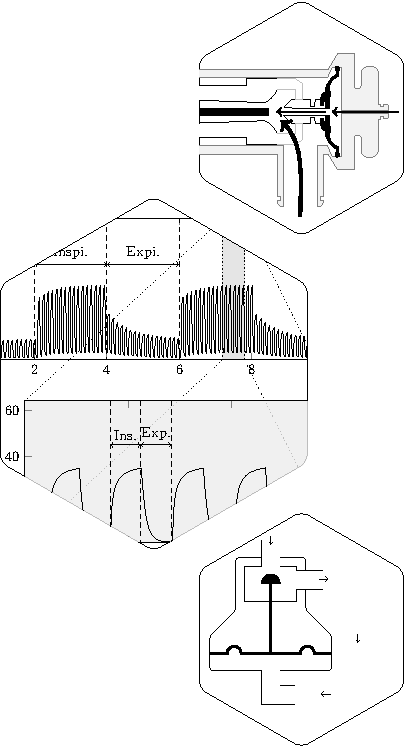
\includegraphics{titlepage/cover}}

\hypersetup{
	pdftitle=Ventilation diffusive convective,
	pdfauthor=Nicolas Blais St-Laurent
}

\begin{document}

%%%%%%%%%%%%%%
% Frontmatter
%%%%%%%%%%%%%%
\frontmatter
\maketitle

\cleardoublepage
\tableofcontents
%\listoftables
\clearpage
\listoffigures
%\listofexercices

%%%%%%%%%%%%%%
% Mainmatter
%%%%%%%%%%%%%%

\mainmatter
\chapter{Introduction}

Le VDR-4 est un appareil de ventilation à haute fréquence conçu à la fin des années 1980 par l'inventeur américain Forest Morton Bird. 
Il a été conçu en tant qu'appareil de ventilation universel, capable de ventiler adéquatement n’importe quel poumon humain, sain ou gravement malade, de la clientèle néonatale à la clientèle adulte. 
Son développement a été motivé par le constat que la ventilation mécanique en pression positive conventionnelle (c’est-à-dire basée sur un volume courant et une fréquence physiologiques) était peu adaptée à la ventilation d'un patient présentant une pathologie pulmonaire inhomogène (MPOC, pneumonie, brûlure d’inhalation, SDRA, etc.).

Outre le type singulier de ventilation qu’il délivre \footnote{Voir section~\ref{sec:particularite}}, le VDR-4 se distingue aussi par son fonctionnement entièrement pneumatique. Ceci lui confère l'avantage d’être entièrement indépendant de toute source d'alimentation électrique. En contrepartie, l'appareil a des capacités de monitorage très limitées.

\section{Vocabulaire}

\begin{description}
	\item[Convection:] Déplacement d'un volume de gaz. Lors de la ventilation
	<<conventionnelle>>, les échanges gazeux entre le circuit du ventilateur et
	les bronchioles terminales se font par convection. On peut donc parler de
		ventilation convective\cite{West2017}.  
	\item [Diffusion:] Déplacement des molécules d’un gaz à l’intérieur d’un mélange gazeux. Les molécules d’un gaz diffusent en suivant leur gradient de concentration.
	\item [Hertz:] Unité de mesure de fréquence correspondant à un cycle par seconde ou soixante cycles par minute.
	\item [Iatrogène:] Causé par la thérapie.
	\item [Percussion:] Bref jet de gaz à haute vélocité.
	\item [Pression motrice:] Dans un contexte de ventilation par VDR-4, on désigne pression motrice la différence entre la pression moyenne à l’inspiration et la pression moyenne à l’expiration.
	\item [Pression partielle:] Pression exercée par les molécules d’un gaz à l’intérieur d’un mélange gazeux.
\end{description}

\section{Notions de ventilation à haute fréquence}

Ce qui caractérise la ventilation à haute fréquence est l'administration de volumes courants inférieurs au volume de l'espace mort anatomique du patient. Les échanges gazeux entre les alvéoles et le circuit de ventilation s'y font selon un ensemble de mécanismes différents. À ce jour, l'influence respective de chacun de ces mécanismes reste encore à élucider\cite{Pillow2005}.

\subsection{Oxygénation lors de la ventilation à haute fréquence}

Les facteurs influençant l'oxygénation lors de la ventilation à haute fréquence sont, à toute fin pratique, les mêmes que pour la ventilation convective.

Dans l'absolu, l'oxygénation du sang est proportionnelle à la pression partielle d'oxygène dans les alvéoles. Les trois principales variables influençant cette pression partielle sont:
la concentration d'oxygène dans l'air insufflé,
la pression alvéolaire moyenne,
la concentration alvéolaire de gaz carbonique.

\subsection{Relation fréquence-volume-ventilation}

Ce qui limite les volumes courants en ventilation à haute fréquence est le peu de temps disponible pour chaque cycle respiratoire. Ce temps est d'autant plus court que la fréquence est élevée. 

$$ {T_{cycle}}_{(s)} = \frac{60}{Freq._{(cycle/min)}}$$

En conséquence, une diminution de la fréquence entrainera une augmentation du volume courant en laissant plus de temps à la pression pour s'équilibrer entre le circuit et les alvéoles. Inversement, une augmentation de la fréquence entrainera une diminution du volume courant.

Ainsi, en ventilation à haute fréquence, une diminution de la fréquence favorise une plus grande élimination du $CO_2$.

Il a été démontré que la fréquence est un paramètre très important pour l'élimination du $CO_2$ en ventilation à haute fréquence\cite{Pillow2005}.

\section{Particularité du VDR-4}
\label{sec:particularite}
Le VDR-4 se distingue des autres appareils de ventilation à haute fréquence par l’alternance (à basse fréquence) entre deux (voire même trois) amplitudes de percussion. Il en résulte une alternance entre deux pressions moyennes. Les échanges gazeux lors de ce type de ventilation seront, par conséquent, à la fois le résultat du déplacement de volumes d’air (convection) et de l’accélération de la diffusion propre à la ventilation à haute fréquence\marginpar{Reformuler ?}.

\begin{figure}
	\tikzsetnextfilename{fig-lfhf}

\pgfplotsset{
	lfhf/.style={
		height = 0.42 \textheight,
		enlarge y limits = {value=0.9, upper},
		enlarge x limits = false
		}
}

\tikzset{
	zoomline/.style={
		opacity=1,
		dotted
	},
	plage/.style={
		<->
	}
}

\def\zstart{7.2}
\def\zend{7.8}
\newcommand{\istart}{2}
\newcommand{\tic}{2}
\newcommand{\pstart}{7.365}
\newcommand{\tip}{0.059}

\begin{tikzpicture}
	\begin{groupplot}[
			group style={
				group size=1 by 2,
				y descriptions at=edge left,
				xlabels at=edge bottom
				},
				ylabel=Pression (hPa),
				xlabel=Temps (s),
				max space between ticks=40,
			]
		\nextgroupplot[lfhf, width=\textwidth, height=5cm]

		\addplot []table[x=time, y=Pao] {dat/simvent1.dat};


		\coordinate (PSO) at (axis cs:\zstart,0);
		\coordinate (PSE) at (axis cs:\zend,0);
		\coordinate (PNO) at (axis cs:\zstart,\pgfkeysvalueof{/pgfplots/ymax});
		\coordinate (PNE) at (axis cs:\zend,\pgfkeysvalueof{/pgfplots/ymax});

		\draw [plage](axis cs:\istart,45) -- (axis cs:\istart + \tic, 45) node[midway, above] {Inspi.};
		\draw [plage](axis cs:\istart + \tic,45) -- (axis cs:\istart + 2*\tic, 45) node[midway, above] {Expi.};

		\draw [dashed] 
		(axis cs: \istart,\pgfkeysvalueof{/pgfplots/ymax}) -- (axis cs:\istart,0)
	 	(axis cs: \istart + \tic,\pgfkeysvalueof{/pgfplots/ymax}) -- (axis cs:\istart + \tic,0)
		(axis cs: \istart + 2 *\tic,\pgfkeysvalueof{/pgfplots/ymax}) -- (axis cs:\istart + 2*\tic,0);

		%\fill [opacity=0.15] (PSO) rectangle (PNE);
		\draw [zoomline] (PSO) rectangle (PNE);


		\nextgroupplot[lfhf,
				max space between ticks=80,
				width=0.75\textwidth,
				height=5cm,
				axis background/.style={fill=gray!15, opacity=0.8},
				]
		\addplot [restrict x to domain=\zstart:\zend]table[x=time, y=Pao] {dat/simvent1.dat};

		\coordinate (ZNO) at (axis cs:\zstart,\pgfkeysvalueof{/pgfplots/ymax});
		\coordinate (ZNE) at (axis cs:\zend,\pgfkeysvalueof{/pgfplots/ymax});
		\coordinate (ZSO) at (axis cs:\zstart,\pgfkeysvalueof{/pgfplots/ymin});
		\coordinate (ZSE) at (axis cs:\zend,\pgfkeysvalueof{/pgfplots/ymin});


		\draw [dashed] 
		(axis cs: \pstart,\pgfkeysvalueof{/pgfplots/ymax}) -- (axis cs:\pstart,0)
		(axis cs: \pstart + \tip,\pgfkeysvalueof{/pgfplots/ymax}) -- (axis cs:\pstart + \tip,0)
		(axis cs: \pstart + 2 *\tip,\pgfkeysvalueof{/pgfplots/ymax}) -- (axis cs:\pstart + 2*\tip,0);
		\draw [plage] (axis cs:\pstart,45) -- (axis cs:\pstart + \tip, 45) node[midway, above] {Ins.};
		\draw [plage](axis cs:\pstart + \tip,45) -- (axis cs:\pstart + 2*\tip, 45) node[midway, above] {Exp.};

	\end{groupplot}

	\begin{scope}[on background layer]
		%\fill [opacity=0.03](ZNO) -- (PNO) -- (PNE) -- (ZNE) -- (ZNO);
		%\fill [opacity=0.03](ZSO) -- (PSO) -- (PNO) -- (PNE) -- (PSE) -- (ZSE) -- (ZSO);
		\fill [opacity=0.1](PSO) -- (PNO) -- (PNE) -- (PSE);
		%\fill [opacity=0.05](ZNE) -- (PNE) -- (PSE) -- (ZSE) -- (ZNE);
		\draw [zoomline](ZNO) -- (PNO) (PNE) -- (ZNE) ;
		\draw [zoomline](ZSO) -- (PSO) (PSE) -- (ZSE) ;
	\end{scope}

\end{tikzpicture}

	\caption{L’alternance entre deux amplitudes de percussions donne une apparence typique au tracé de la pression à l'ouverture des voies aériennes lors de la ventilation avec un VDR-4. Les phases inspiratoires et expiratoires à basse fréquence (courbe du haut) sont composées d’une succession d’inspirations et d’expirations à haute fréquence (courbe du bas).}
\end{figure}

\def\knobshow#1{%
\marginpar{%
	\centering
	\begin{tikzpicture}
\pic [pic text=#1, scale=1.5] {aknob};
\end{tikzpicture}%
}}

\chapter{Paramètres de ventilation}

Le réglage des paramètres de ventilation se fait en ajustant l’ouverture de
valves sur le module de contrôle. Les valves du module de contrôle sont
identifiées par le principal paramètre visé par le réglage. Cependant, le
réglage de l’ouverture d’une valve entraine presque toujours la modification
d’au moins deux paramètres. Un code de couleurs identifie les valves en
fonction du type de paramètre visé par son réglage.  

\section{Paramètres d’amplitude}

Une amplitude de percussion différente peut être réglée pour chacune des trois
phases du cycle de convection (basse fréquence).  Ces trois réglages sont
identifiés par la couleur verte sur le module de contrôle. 

\subsection{Amplitude des percussions à l’inspiration (phase haute)}

Il s’agit du paramètre de base à partir duquel sont réglés les deux autres
paramètres d’amplitude. Cela signifie qu’une modification de ce paramètre
entrainera une modification dans la même direction des deux autres amplitudes.
Cette amplitude est réglée au moyen de la valve identifiée Debit pulse.
\knobshow{D}

\subsection{Amplitude des percussions à l’expiration (phase basse)}

L’amplitude des percussions pendant l’expiration convective est réglée par
comparaison à celle pendant l’inspiration convective. Cela signifie qu’une
modification de l’amplitude à l’inspiration entrainera une modification de
l’amplitude à l’expiration. Par contre, l’amplitude à l’inspiration ne sera pas
affectée par une modification de celle à l’expiration. Cette amplitude est
réglée au moyen de la valve identifiée CPAP oscillante.
\knobshow{O}

\subsection{Amplitude de percussion augmentée (troisième phase)}

Lorsqu’elle est activée, la troisième phase commence 0,8 seconde après le début
de l’inspiration convective (voir Figure 10). Il en résulte une inspiration en
deux temps. Cette amplitude est réglée au moyen de la valve identifiée pression
de convection. Ce paramètre n’est pas utilisé dans le protocole clinique en
vigueur au CHUM.
\knobshow{C}

\begin{figure}
\caption{Tracé de la pression à l'ouverture des voies aériennes. On peut
observer une augmentation de la pression 0.8 secondes après le début de
l’inspiration.}
\end{figure}

\begin{table}
	\begin{tabular}{l l}
		\hline
		Paramètre & Désignation sur l’appareil\\
		\hline
		Amplitude à l’inspiration (phase haute) & DEBIT PULSE\\
		Amplitude à l’expiration (phase basse) & CPAP OSCILLANTE\\
		Amplitude augmentée (troisième phase) & PRESSION DE CONVECTION\\
\hline
	\end{tabular}
	\caption{Désignation des contrôles relatifs à l'amplitude de percussion.}
\end{table}

\section{Paramètres de cyclage à haute fréquence}

Les valves contrôlant le cyclage à haute fréquence sont identifiées par la
couleur grise sur le module de contrôle.  Bien que les deux boutons permettant
de régler le cyclage à haute fréquence soient désignés «FRÉQUENCE DE
PERCUSSION» et «RATIO i:e» sur l’appareil, il s’avère que chacun de ces deux
\knobshow{i}
réglages influence la fréquence.  En fait, le bouton «FRÉQUENCE» modifie le
temps inspiratoire des percussions sans modifier le ratio i:e. Il en résulte
donc une modification de la fréquence avec un ratio i:e constant.  Quant au
bouton « RATIO i:e » il ajuste le ratio i:e sans modifier le temps
inspiratoire. Il en résulte qu’une modification du ratio i:e modifie aussi la
fréquence de percussion.
\knobshow{e}

\section{Paramètres de cyclage à basse fréquence}

Le cyclage à basse fréquence se règle en ajustant un temps inspiratoire et un
temps expiratoire.  La fréquence et le ratio inspiration : expiration
résulteront des temps inspiratoire et expiratoire réglés. Les valves contrôlant
le cyclage à basse fréquence sont identifiées par la couleur noire sur le
module de contrôle.

\section{PEP non oscillante}

La fonction PEP non oscillante (DEMAND CPAP / PEEP) est identifiée par un
bouton de couleur jaune.  Cette fonction est destinée à réduire le travail
respiratoire lors d’essai de respiration spontanée. Elle est généralement
désactivée lors de la percussion. Lorsqu’elle est activée, un débit continu est
injecté dans le phasitron. Ce débit, qui sera amplifié par le phasitron,
facilite l’inspiration et maintient une pression positive à l’expiration (en
maintenant le tube de venturi en position partiellement avancée).  

\section{Autres paramètres}

\subsection{Pression de travail}

La pression de travail est la pression à laquelle les gaz entrent dans le
circuit de logique pneumatique. Celle-ci influence à la fois l’amplitude des
percussions et les paramètres de cyclage. Chez l’adulte, on utilise
généralement la pression la plus élevée pouvant être atteinte (plus ou moins 40
\psi, selon la source d’alimentation en gaz pressurisé).


\subsection{Nébulisation}

Active ou désactive le débit destiné à actionner le nébuliseur (plus ou moins
20 l/min). Actif même lorsque la percussion est arrêtée. 

\subsection{Marche arrêt}

S’applique à la percussion seulement. Toutes les autres fonctions
(nébulisation, PEP non percussive, monitorage) demeurent actives.

\section{Interactions des paramètres}

Pour faire une règle simple, on peut dire, sans trop exagérer, que n'importe
quel paramètre peut potentiellement influencer n'importe quel autre paramètre. 

\subsection{Paramètres influençant le cyclage}

Étant donné que l’alternance entre les inspirations et les expirations des
percussions (cyclage haute fréquence)  est contrôlé par des cartouches
pneumatiques, tout paramètre influençant la pression disponible pour actionner
les cartouches peut influencer la fréquence des percussions et leur ratio i:e.
Parmi ces paramètres, on compte entre autres :

\begin{itemize}
\item La pression de travail, 
\item La \fio, 
\item Le réglage d’amplitude des percussions (DEBIT PULSE).
\end{itemize}

Le même principe s’applique au cyclage à basse fréquence (temps inspiratoire et
expiratoire convectif).

\subsection{Influence du ratio i:e des percussions sur les pressions de ventilation}

Le ratio inspiration : expiration (i:e) des percussions a une grande influence
sur les pressions de ventilation. Plus le ratio i:e est élevé, plus les
pressions serons élevées.

\section{Séquence des réglages}

\begin{figure*}
	\centering
\begin{tikzpicture}

	\pic [name=VDR, black!60, scale=0.8] {vdr};

	\begin{scope}[
		every node/.style={
			color=black,
			}
			]
	\node (1) at (VDR-e) {1};
	\node (2) at (VDR-i) {2};
	\node (3) at (VDR-F) {3};
	\node (4) at (VDR-O) {4};
	\node (5) at (VDR-I) {5};
	\node (6) at (VDR-E) {6};
	\end{scope}

	\begin{scope}[
		every node/.style={
			yshift=8mm,
			align=center,
			scale=0.5
			}
			]
	\node at (VDR-e) {RAPPORT\\i/e};
	\node at (VDR-i) {FREQUENCE\\DE PERCUSSION};
	\node at (VDR-F) {DEPIT\\PULSE};
	\node at (VDR-O) {CPAP\\OSCILLANTE};
	\node at (VDR-I) {TEMPS\\INSPIRATOIRE};
	\node at (VDR-E) {TEMPS\\EXPIRATOIRE};
	\end{scope}

	\begin{scope}[
		every path/.style={
			black,
			opacity=0.80,
			line width=0.7mm,
			->
			},
			]
	\draw [] (1) to (2);
	\draw [bend left=27] (2) to (3);
	\draw [bend left=60] (3) to (4);
	\draw [bend left=45] (4) to (5);
	\draw [bend left=45] (5) to (6);
	\end{scope}

\end{tikzpicture}

	\caption{Séquence de réglage des paramètres.}
\end{figure*}

En raison des interactions entre les différents réglages, il est
judicieux de régler en premier les paramètres ayant beaucoup d'influence
sur les autres réglages, ou influençant plusieurs autres réglages.

Ainsi, avant d'effectuer quelque réglage que ce soit, on s'assurera que
la pression de travail est réglée à 40 lb/po\textsuperscript{2} et que la nébulisation est
en fonction. On s'assurera aussi que la PEP non oscillante et
l'augmentation des pressions de convection (3\textsuperscript{e} phase) sont désactivées
(tourné complètement en sens horaire).

Ensuite, étant donné que le rapport \ie\ des percussions (haute
fréquence) influence à la fois la fréquence de percussion et l'amplitude
des percussions (donc les pressions de ventilation), il est judicieux
d'ajuster ce paramètre en tout premier lieu.

Une fois le rapport \ie\ des percussions ajusté,~le temps inspiratoire
des percussions peut être ajusté à n'importe quel moment pour régler la
fréquence de percussion.

Pour les paramètres d'amplitude de percussion, l'amplitude des
percussions pendant l'inspiration influence celle pendant l'expiration.
Il convient donc de toujours ajuster la pression inspiratoire avant la
pression expiratoire.

Finalement, les pressions de ventilation ayant une influence sur le
temps inspiratoire et expiratoire de la convection (basse fréquence),
on attendra d'avoir ajusté les pressions de ventilation avant de régler
avec précision ces deux paramètres.

\chapter{Surveillance clinique}

\section{Données monitorées}

On retrouve à la fois des données mesurées sur le multimètre situé sur
le dessus du module de contrôle et sur le Monitron. Certaines données
sont même affichées aux deux endroits.

\emph{Il est important de noter que pour l'application du protocole de
ventilation du CHUM, c'est toujours les pressions affichées sur le
multimètre du module de contrôle que l'on doit utiliser (moyenne
inspiratoire et moyenne expiratoire).  Les pressions affichées par le Monitron (PEAK PRESSURE et PEEP/CPAP)
sont lues à la crête de l'oscillation et sont par conséquent peu
représentatives des pressions subies par les alvéoles pulmonaires.
}
\def\ptitle#1{\vspace{.4\baselineskip}\textbf{#1}\par\vspace{0.4\baselineskip}}

\begin{framed}
	\ptitle{Données affichées par le Multimètre numérique et par le Monitron. }
	\ptitle{Multimètre du module de contrôle }
	\protochum{Pression inspiratoire moyenne}\\
	\protochum{Pression expiratoire moyenne}\\
	Pression moyenne globale\\
	\protochum{Fréquence de percussion ($F_{perc}$)}

	\ptitle{Monitron}
	\raggedright
	Pression inspiratoire de crête\\
	Pression expiratoire de crête (PEP)\\
	Pression moyenne globale\\
	\protochum{Ti (convection)}\\
	\protochum{Te (convection)}\\
	I:E\\
	F\textsubscript{conv}\\
	\protochum{Fréquence de percussion ($F_{perc}$)}\\
	i:e

	\vspace{0.2\baselineskip}
	{\small *\protochum{}\space \emph{Données utilisées dans le
	protocole clinique du CHUM}}
	\end{framed}


\begin{figure}
	\newcommand{\pexp}{5}
\newcommand{\pins}{18}
\newcommand{\arrpos}{1.06}
\begin{tikzpicture}[
		pressmark/.style={
			draw=gray,
			dashed,
		},
		pline/.style={
			pressmark,
			help lines,
			rounded corners,
			out=0,
			in=180,
			thick
			},
		pcircle/.style={
			pressmark,
			circle,
			inner sep=0.5mm,
			thick
			}
	]

	\begin{axis}[
		width=0.75\textwidth,
		height=5cm,
		name=plot,
		font=\scriptsize,
		try min ticks=6,
		xtick={0,4,8},
		ytick={0,30},
		axis x line=bottom,
		axis y line=middle,
		enlarge y limits={value=0.1, upper},
		enlarge x limits={value=0.05, upper},
		extra y ticks={5, 18},
		extra y tick labels={$P_{ins. moy.}$, $P_{exp. moy.}$},
		extra y tick style={grid=major},
		major grid style={pressmark, thick}
		]

		\addplot [
			black,
			restrict x to domain=0:8,
			] table[x=time, y=Pao] {dat/f300.dat};

		\coordinate (D) at (axis cs: \pgfkeysvalueof{/pgfplots/xmax},\pins);
		\coordinate (B) at (axis cs: \pgfkeysvalueof{/pgfplots/xmax},\pexp);

	\end{axis}

	\pic [opacity=0.99, name=mm, scale=1] at ([xshift=3.2cm, yshift=0cm]plot.east) {multimeter};

		\node [grad] (mmg50) at (mmscreen.north west) {50};
		\node [grad] (mmg0) at (mmscreen.south west) {0};
		\draw [pScale]	(mmg0) -- (mmg50) node [grad, left=0.0mm, pos=0.6, inner sep=0mm] {30};

		\node [below, white, align=left, font=\tiny] at (mmscreen.south) {Percussionaire\\Corporation};

	\node [pcircle] (pmi) at (mmPmi) {\pins};
	\node [pcircle] (pme) at (mmPme) {\pexp};

	\draw [pline] (D) to (pmi);
	\draw [pline] (B) to (pme);
\end{tikzpicture}

	\caption{La pression inspiratoire moyenne et la pression expiratoire moyenne sont affichées sur me multimètre numérique se trouvant sur le dessus du ventilateur.}
\end{figure}

\section{Monitorage du rapport \ie}

On se rappellera que l'affichage du rapport \ie\ sur le Monitron n'est
fonctionnel que lorsque le Ti est plus petit que le Te. Lorsque le Ti
devient plus grand que le Te (rapport inversé), le Monitron affiche en
permanence 1\string: 1.0.

La meilleure façon de juger du rapport \ie\ est alors d'observer
l'apparence de la courbe de pression sur le monitron.

Les éléments à observer sont:

\begin{itemize}
\item
  Durée du Ti (montée de pression et plateau) versus celle du Te (chute
  de la pression) (observer à 1 ou 2 s par écran);
\item
  Présence d'un plateau. Un plateau où la pression plafonne complètement
		est suggestif d'un ratio inversé. Voir Figure~\ref{figie1}, courbe du bas.
  (observer à 1 ou 2 s par écran);
\item
  Espace sous la courbe de pression. L'augmentation de l'espace sous la
  courbe pendant l'inspiration convective est aussi suggestive d'un
  ratio inversé. Elle témoigne d'une diminution de l'amplitude des
  percussions. Voir Figure~\ref{figie8}, courbe du bas. (observer à 5 ou 8 s par
  écran);
\end{itemize}
\begin{figure*}
	\def\iehuit{%
\addplot graphics [
	xmin=0,
	ymin=0,
	xmax=1,
	ymax=60
]}

\begin{tikzpicture}

\begin{groupplot}[
		group style={
			group size=1 by 2,
			xlabels at=edge bottom
		},
		enlargelimits=false,
		height=4cm,
		width=\textwidth,
		xtick={0, .25, .5, .75, 1},
		xlabel=Temps (s),
		ylabel=Pression (hPa)
]

\nextgroupplot
\iehuit {img/509-gray.jpg};

\nextgroupplot
\iehuit{img/828-gray.jpg};

\end{groupplot}
\end{tikzpicture}

	\caption{Rapport \ie\ adéquat (en haut) et rapport \ie\ inversé (en
	bas). On observe sur le tracé du bas un Te trop court ne permettant pas
	à la pression de redescendre entre chaque percussion. La pression
	d'équilibre est donc rapidement atteinte à la percussion suivante. Il en
	résulte une faible amplitude de variation de pression à chaque
	percussion. Vitesse de défilement à 1 s par écran.}
	\label{figie1}
\end{figure*}

\begin{figure*}
	\def\iehuit{%
\addplot graphics [
	xmin=0,
	ymin=0,
	xmax=8,
	ymax=60
]}

\begin{tikzpicture}

\begin{groupplot}[
		group style={
			group size=1 by 2,
			xlabels at=edge bottom
		},
		enlargelimits=false,
		height=4cm,
		width=\textwidth,
		xtick={0, 2, 4, 6, 8},
		xlabel=Temps (s),
		ylabel=Pression (hPa)
]

\nextgroupplot
\iehuit {img/329-gray.jpg};

\nextgroupplot
\iehuit{img/629-gray.jpg};

\end{groupplot}
\end{tikzpicture}

	\caption{Rapport \ie\ adéquat (en haut) et rapport \ie\ inversé (en
	bas). On observe une diminution de l'amplitude de percussion sur le
	tracé du bas. Vitesse de défilement à 8 s par écran.}
	\label{figie8}
\end{figure*}

\section{Alarme}\index{alarme}

\subsection{Alarmes du module de contrôle}

\subsubsection*{Alarme du mélangeur air-oxygène}

Il s'agit d'une alarme pneumatique se déclenchant lorsque le mélangeur
perd son alimentation en air ou en oxygène. Il n'y a pas de fonction
\emph{silence} ou \emph{réarmer~}: l'alarme s'arrête automatiquement
lorsque l'alimentation des deux gaz est rétablie.

\subsubsection{Alarme de surpression}\index{alarme!de surpression}

Il s'agit d'une alarme pneumatique se déclenchant lors d'une surpression
dans le module de contrôle. Son déclenchement entraine une chute de la
pression délivrée. Une fois la cause corrigée, il faut réarmer l'alarme
(bouton poussoir rouge) pour que la ventilation reprenne normalement.

Au réglage le plus sensible (rotation en sens antihoraire) l'alarme se
déclenche lorsque la pression dans le circuit avoisine les 80 $cmH_2O$.

Lorsque cette alarme se déclenche, il faut en premier lieu suspecter un
réglage inadéquat (par exemple fonction \emph{PRESSION DE CONVECTION} ou
\emph{PEP non oscillante} activées ou fréquence de percussion inférieure
à 100) ou une tubulure blanche coincée.

Il est improbable qu'une condition clinique (par exemple toux ou
résistances augmentées) entraine l'activation de cette alarme.

\subsubsection{Alarme de déconnexion}
\index{alarme!de déconnexion}

Il s'agit d'un module indépendant situé sur le côté de l'appareil et
alimenté par une batterie. Cette alarme se déclenche lorsqu'aucune
pression n'est détectée dans le circuit pour une période donnée. Cette
période peut (en théorie\ldots{}) être ajustée au moyen de la roulette
noire.

\subsection{Alarmes du Monitron}

\subsubsection*{Alarme de pression haute}%

Cette alarme se déclenche dès que la pression dans le circuit est
supérieure à la limite réglée. La valeur du réglage est indiquée par une
ligne rouge dans la zone de graphiques.

Son réglage répond même logique que l'alarme de pression haute en
ventilation conventionnelle (par exemple 10 $cmH_2O$ de plus que la
pression de crête actuelle). Il faut cependant se rappeler que le
déclenchement de l'alarme n'interrompt pas la ventilation étant donné
que le Monitron et le module de contrôle sons indépendants l'un de
l'autre.

\subsubsection*{Alarme de pression basse}

Cette alarme s'active lorsque la pression dans le circuit est inférieure
au seuil réglé pour plus de 6 s (alarme visuelle) et 12 s (alarme
sonore).

Il est à noter qu'une fois la pression rétablie, l'alarme continue à
sonner tant qu'elle n'a pas été réarmée.

\section{Situations particulières}

\subsection{Obstruction de la sonde}\index{obstruction!de la sonde s'intubation}

Étant donné l’absence de monitorage du débit, il est nécessaire de faire preuve
d’une vigilance accrue afin de détecter cette complication. Une obstruction
importante de la sonde peut se manifester par :
		
\begin{itemize}
	\item Une augmentation des pressions de ventilation en l’absence de
	modification des réglages. L’augmentation de la pression à l’inspiration se
	fera de façon plus abrupte, 
	\item Une détérioration des échanges gazeux.
\end{itemize}

La perméabilité de la sonde peut être évaluée en y descendant un cathéter
d’aspiration, que ce soit en cas de doute ou sur une base régulière.  Si
l’abondance des sécrétions est problématique, le ballonnet du tube endotrachéal
peut être partiellement dégonflé pour permettre à celles-ci de remonter dans
l’oropharynx du patient. L’amplitude des percussions devra alors être réajustée
à la hausse pour compenser la fuite créée.

\begin{figure}
\centering
	\begin{tikzpicture}
		\begin{groupplot} [
				group style={
					group size=2 by 1,
					ylabels at=edge left,
				},
				ylabel=$P_{circ.} (hPa)$,
				xlabel=Temps (s),
				width=0.5\textwidth,
				restrict x to domain=1.5:4,
				ymax=40,
				every axis plot post/.style={
					mark=none
				}
			]
			\nextgroupplot [title=Résistances normales]
			\addplot [] table[x=time, y=Pao] {dat/raw5.dat};

		 \nextgroupplot [title=Résistances augmentées]
			\addplot [] table[x=time, y=Pao] {dat/raw15.dat};
		\end{groupplot}
	\end{tikzpicture}

\caption{Modification de l'apparence de la courbe de pression suite à une
augmentation des résistances. Lorsque les résistances sont normales (à gauche),
on observe une augmentation graduelle des pressions lors de l’inspiration.
Cette augmentation correspond à l’augmentation de la pression alvéolaire.
Lorsque les résistances sont élevées, les pressions sont élevées dès le début
de l’inspiration et restent stable au cours de celle-ci.}
\index{résistances!augmentées}
\end{figure}

\subsection{Fuite ou déconnexion}\index{fuite}\index{déconnexion}

Une fuite entre le phasitron et le patient ou au niveau du tube endotrachéal se
manifestera par une diminution des pressions mesurées en l’absence de
modification des réglages. La courbe de pression aura une apparence atténuée.
Une fuite dans le circuit d’humidification n’aura pas d’influence sur les
pressions de ventilations. Elle pourra, par contre, modifier la concentration
en oxygène du mélange gazeux administré au patient (appel d’air ambiant),
entrainant une hypoxémie+.


%\chapter{Stratégies de ventilation}
%\chapter{Données probantes}
%\chapter{Au coeur de la bête}

%%%%%%%%%%%%%%
% Backmatter
%%%%%%%%%%%%%%

\begin{appendices}

\newgeometry{
	includeall,
	margin=0.8in,
	marginparwidth=0in,
	marginparsep=0in
}

\chapter{Protocole clinique du Centre hospitalier de l'Université de Montréal}
%\includepdf[pages=-]{../formationvdr4/documents/pub/INH-PROT-05-01.pdf}

\titleformat{\chapter}[display]{\normalfont\huge\bfseries}{\chaptertitlename\ \thechapter}{20pt}{\Huge}   
\titlespacing*{\chapter}{0pt}{-50pt}{40pt}

\chapter{Horaire type d'une formation}
\section*{Journée 1}
\begin{horaire}{450}
	\thispagestyle{empty}
	\activite{15}{Accueil des participants}
	\activite{10}{Objectifs de la formation}
	\activite{30}{Exploration des acquis}
	\activite{30}{Revue de la littérature}
	\activite{30}{Montage du circuit et vérification pré-utilisation}
	\activite{30}{Théorie relative au circuit}

	\hline
	\activite{15}{Pause}
	\hline

	\activite{30}{Paramètres de base, moniteurs et alarmes}
	\activite{45}{Position par défault et interaction i:e}
	\activite{30}{Théorie relative au rapport i:e}

	\hline
	\activite{60}{Diner}
	\hline

	\activite{40}{Évaluation du ratio i:e}
	\activite{60}{Expérimentation/théorie supplémentaire}
	\hline
	\activite{15}{Pause}
	\hline

	\activite{40}{Jeux des erreurs}
	\activite{15}{Conclusion}
\end{horaire}

\section*{Journée 2}

\begin{horaire}{450}
	\activite{60}{Retour sur la journée 1 et réponses aux questions}
	\activite{180}{Protocole de ventilation}
	\hline
	\activite{60}{Dîner}
	\hline
	\activite{180}{Mises en situations}
	\activite{15}{Conclusion}
\end{horaire}


\end{appendices}
\restoregeometry

\backmatter

\printbibliography
\printindex
\end{document}
